\documentclass[twocolumn, final]{elsarticle}

\usepackage{lineno,hyperref}
\usepackage{graphicx}

\modulolinenumbers[5]

\journal{Journal of \LaTeX\ Templates}
%%%%%%%%%%%%%%%%%%%%%%%
%% Elsevier bibliography styles
%%%%%%%%%%%%%%%%%%%%%%%
%% To change the style, put a % in front of the second line of the current style and
%% remove the % from the second line of the style you would like to use.
%%%%%%%%%%%%%%%%%%%%%%%

%% Numbered
%\bibliographystyle{model1-num-names}

%% Numbered without titles
%\bibliographystyle{model1a-num-names}

%% Harvard
%\bibliographystyle{model2-names.bst}\biboptions{authoryear}

%% Vancouver numbered
%\usepackage{numcompress}\bibliographystyle{model3-num-names}

%% Vancouver name/year
%\usepackage{numcompress}\bibliographystyle{model4-names}\biboptions{authoryear}

%% APA style
%\bibliographystyle{model5-names}\biboptions{authoryear}

%% AMA style
%\usepackage{numcompress}\bibliographystyle{model6-num-names}

%% `Elsevier LaTeX' style
\bibliographystyle{elsarticle-num}
%%%%%%%%%%%%%%%%%%%%%%%

\begin{document}
\begin{frontmatter}
\title{.............................................}

%% Group authors per affiliation:
\author{........................................}
\address{Istituto Nazionale di Ricerca Metrologica (I.N.Ri.M.), Strada delle Cacce, 91, 10135 Torino, ITALY}

\begin{abstract}

The combined capability to inject, manipulate and detect spin polarized currents in bilayers formed by a non magnetic conductor with a large 
spin Hall effect (i.e. Pt) and a magnetic insulator Yttrium Iron Garnet (i.e. YIG) represents a milestone in the field of spintronics. This paper 
presents theoretical predictions and a possible mechanism to excite  self-oscillation induced by the spin Hall torque. The spin Hall torque is 
caused by the nonequilibrium magnetization (i.e. spin accumulation) occurring at the interface between the magnetic conductor and a 
magnetic insulator  layer and it may generate magnetization dynamics in the ferrimagnet \cite{collet2016generation}. The microscopic origin 
of this effect has been searched in the transmission of a spin current through the Pt/YIG interface \cite{tserkovnyak2002spin}. However,  
this effect represents a conversion between a DC pure spin current into an AC magnetization dynamics at heavy-metal magnetic-insulator 
interface. To this aim, it is appropriate to employ the nonequilibrium thermodynamic approach originally developed by Johnson and Silsbee 
to describe the joined transport of heat, electric charge and magnetization current \cite{johnson1987thermodynamic}. The theory here 
presented is a possible generalization of the scalar one recently applied in.\cite{basso2016nonequilibrium, basso2016thermodynamic}. 
\end{abstract}

\begin{keyword}
spin hall torque \sep magnetic moment \sep magnetic conductor \sep spin waves \sep nonequilibrium magnetization 
\MSC[2017] 00-01\sep  99-00
\end{keyword}
\end{frontmatter}
\linenumbers

\section{Thermodynamic Model}
In order to extend the approach of \cite{johnson1987thermodynamic, basso2016nonequilibrium, basso2016thermodynamic} to vector 
magnetization $\mathbf{M}$, the continuity equation for a ferromagnetic material with precession is therefore written as:

%===================================================================================
\begin{equation}
\label{equation:continuity_equation}
\partial_t\mathbf{M}+ \nabla\mathbf{J}_{\mathbf{M}}=-\mu_0\gamma_L\mathbf{M}\times\mathbf{H}_{\mathrm{\scriptstyle{eff}}}^* 
+\tau_{\mathrm{\scriptstyle{M}}}^{-1}\mathbf{H}_{\mathrm{\scriptstyle{eff}}}^*
\end{equation}
%===================================================================================

Here we consider the equation where the left-hand side of the Eq.\ref{equation:continuity_equation} contains the local variation of magnetization and the divergence of the  
magnetization current $\mathbf{J}_{\mathbf{M}}$ and the right-hand side includes a source/sink terms proportional to the thermodynamic effective field $\mathbf{H}
_{\mathrm{\scriptstyle{eff}}}^*$ expressing the distance from equilibrium and characterized by the damping coefficient $\alpha$, and a precessional term written in the Landau-
Lifshitz style. In the previous equation, $\gamma_{\mathrm{\scriptstyle{L}}}$ is the gyromagnetic ratio, $\mathbf{M}$ its amplitude. The proportionality of the magnetic 
moment current is taken into account by an appropriate constitutive relation  $\mathbf{J}_{\mathbf{M}}=\mu_0\sigma_{\mathrm{\scriptstyle{M}}}\nabla\cdot\mathbf{H}
_{\mathrm{\scriptstyle{eff}}}^*$ with $\mathbf{J}_{\mathbf{M}}$  the gradient of the potential $\nabla\cdot\mathbf{H}^*$ and the conductivity tensor $
\sigma_{\mathrm{\scriptstyle{M}}}$. In particular, Eq.\ref{equation:continuity_equation} reduces to the case considered in \cite{basso2016nonequilibrium}, 
\cite{basso2016thermodynamic} if the precessional term  $\mathbf{M} \times\mathbf{H}^*_{\mathrm{\scriptstyle{eff}}}$ is set equal to zero. To study the spin Hall torque 
problem, Eq.\ref{equation:continuity_equation} shall be solved for $\mathbf{H}^*_{\mathrm{\scriptstyle{eff}}}$ and thus it is necessary to add the constitutive relations 
between $\mathbf{J}_{\mathbf{M}} $ and $\nabla\cdot\mathbf{H}^*_{\mathrm{\scriptstyle{eff}}}$, which is the thermodynamic driving force for the magnetization 
currents \cite{basso2016nonequilibrium, basso2016thermodynamic}. The conduction of the magnetic moment in ferromagnets can be caused by spin polarized electrons (in metals) and 
spin waves. In both cases the symmetry is broken by the presence of the spontaneous magnetization. Here we limit to the case in which the magnetic moment can be transferred by 
means of spin waves. The spin wave picture is applied both for  general magnetization or to the cases in which the magnetization has only a small deviation from its equilibrium.

%===================================================================================

\begin{figure}[htbp]
\begin{center}
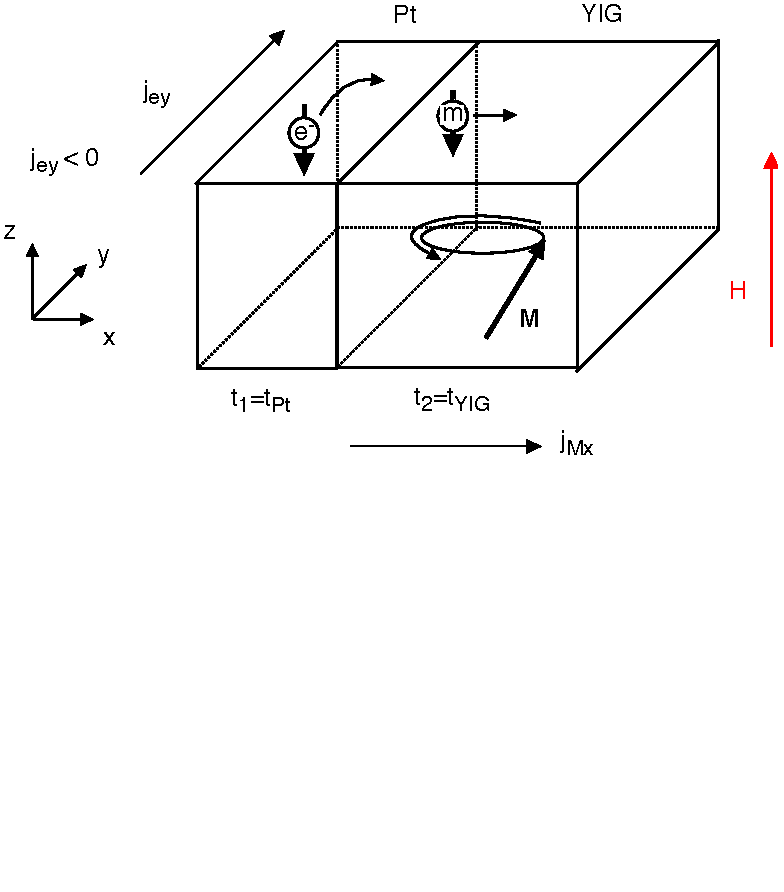
\includegraphics[width=8cm]{scheme.pdf}
\caption{representation of a magnetization and an applied external and spin orbit torque fields}
\label{scheme}
\end{center}
\end{figure}

%===================================================================================

The effect of the spin accumulation is to reduce the value of the magnetization's module $|\mathbf{M}|$ during this time the 
magnetization is directed along the $z-$axis then projecting Eq.\ref{equation:continuity_equation} in the direction of the magnetization  
(i.e.  scalar multiplying  the Eq.\ref{equation:continuity_equation} with the vector $\mathbf{e}_z)$ we have the following diffusion 
equation  for the modules of the magnetization $\mathbf{M}$: 

%===================================================================================

\begin{equation}
\tau_\mathrm{\scriptstyle{M}}\frac{\partial \mathbf{|M|}}{\partial t} + l_\mathrm{\scriptstyle{M}}^2 \nabla^2 \mathrm{H}_{\mathrm{\scriptstyle{z}}}^*  
= \mathrm{H}_{\mathrm{\scriptstyle{z}}}^* 
\end{equation}
%===================================================================================

In the direction perpendicular to the magnetization by cross multiplying the Eq.\ref{equation:continuity_equation} with the vector $-\mathbf{m}\times(\mathbf{m}\times$ we can 
rewrite Eq.\ref{equation:continuity_equation} as

%===================================================================================

\begin{equation}
\label{EQ:d&p_t}
\frac{\partial  \mathbf{m}}{\partial  t} +\nabla\mathbf{J}^{\perp}_{\mathbf{M}}= -\mu_0\gamma_L \, \mathbf{m} \times \left( \mathbf{H}_\mathrm{eff}^{*\perp}+\alpha \mathbf{m} \times \mathbf{H}_\mathrm{eff}
^{*\perp}\right)
\end{equation}
%===================================================================================

where $\mathbf{m}$ is the magnetization direction $\mathbf{m} = \mathbf{M}/\mathrm{M}$ and $\alpha = (\mu_0\gamma_L M \tau_{\mathrm{M}})^{-1}$. In the previous equation only the 
component of $\mathbf{H}_\mathrm{eff}^*$ perpendicular to $\mathbf{M}$ is active . 

\section{Spin Orbit Torque}

The spin Hall torque effect is realized in Pt/YIG systems in which the Pt is the spin Hall conductor able to inject a magnetic moment current into YIG. A constant field along the $z-$direction  is applied to 
YIG. As a result, a potential is generated in YIG by the absorption of the current. To solve the problem one first solve the transport of magnetic moment current along the $z-$direction axis. We take the 
applied field along $z-$direction only and there no applied field in the plane. The equation for $z-$direction component is the simple diffusion one. 

%===================================================================================

\begin{equation}
\nabla\mathbf{J}^{\perp}_{\mathbf{M}}=\tau^{-1}\mathrm{H}^*_{\mathrm{\scriptstyle{z}}}\mathbf{e}_z= \tau^{-1}_\mathrm{M}\mathbf{H}_{\mathrm{\scriptstyle{sot}}}(x)
\end{equation}
%===================================================================================

Ones derived this result we can plug it into the full equation

\section{Self Oscillations}

The spin Hall torque effects  realized in Pt/YIG systems in which the Pt is the spin Hall conductor able to inject a magnetic moment current into YIG. A constant field along the $z-$direction is applied to YIG. As a result, a potential 
$H^*_z$ is generated in YIG by the absorption of the current. To solve the problem one first solve the transport of magnetic moment current along the $z-$ axis. We take the applied field along $z$ only, $H_z$, and there no applied field 
in the plane. The equation for $z-$ component is the simple diffusion one. The solution is given in \cite{basso2016thermodynamic} and shows that the divergence of the current is an extra term (the spin orbit torque term)

%===================================================================================
\begin{equation}
\nabla \cdot \mathbf{J}_{\mathbf{M}} = \tau^{-1}_{{\mathrm{\scriptstyle{M}}}}\mathbf{H}_{\mathrm{\scriptstyle{sot}}}(x)
\end{equation}
%===================================================================================

where 

%===================================================================================

\begin{equation}
\mathbf{H}_{\mathrm{\scriptstyle{sot}}}(x) = - v_{\mathrm{\scriptstyle{eff}}} \frac{\cosh((x-t_{\mathrm{\scriptstyle{YIG}}})/l_{\mathrm{\scriptstyle{YIG}}})}{v_2 
\sinh(t_{\mathrm{\scriptstyle{YIG}}}/l_{\mathrm{\scriptstyle{YIG}}})} \frac{j_{MS}}{v_{\mathrm{\scriptstyle{Pt}}}} \tanh(t_{\mathrm{\scriptstyle{Pt}}}/(2 l_{\mathrm{\scriptstyle{Pt}}}))
\mathbf{e}_z
\end{equation}
%===================================================================================

After having derived this result we can plug it into the full equation and then project it on the plane perpendicular to the magnetization direction. With the applied field, $\mathbf{H}_{a}$, along $z$, the 
dynamic equation for the magnetization direction $\mathbf{m} $  normalized to $\tau=\mu_0\gamma_{\mathrm{\scriptstyle{L}}}\mathrm{M}_{\mathrm{\scriptstyle{s}}}$


%===================================================================================

\begin{equation}
\label{equation:dimensionless_lle}
\frac{\partial \mathbf{m}}{\partial  \tau}=-\mathbf{m} \times \left\{ \mathbf{h}_{\mathrm{\scriptstyle{a}}}+\alpha \mathbf{m} \times[ \mathbf{h}_{\mathrm{\scriptstyle{a}}}-\mathbf{h}
_{\mathrm{\scriptstyle{sot}}}(x)\right]\}
\end{equation}
%===================================================================================

 Hoever expanding in Tylor series up to the first zero order of $t_{\mathrm{\scriptstyle{YIG}}}/l_{\mathrm{\scriptstyle{YIG}}}$  and  $\mathbf{H}_{\mathrm{\scriptstyle{sot}}}(x) =v_1^{-1} 
 J_{\mathrm{\scriptstyle{MS}}}\tanh(t_{\mathrm{\scriptstyle{Pt}}}/2 l_{\mathrm{\scriptstyle{Pt}}}) $the threshold for 
 auto oscillations at  $\mathbf{H}_{a}=\mathbf{H}_{\mathbf{\scriptstyle{sot}}}$, 
 
in this condition the magnetization $\boldmath{m}$  may be driven to an instability leading to self oscillations.  

\section*{References}

\bibliography{bibpaper}

\end{document}
